\documentclass[11pt]{article}

\usepackage[a4paper,margin=25mm]{geometry}
\usepackage{amsmath,amssymb}
\usepackage{siunitx}
\usepackage{booktabs}
\usepackage{hyperref}
\usepackage[nameinlink,noabbrev]{cleveref}
\usepackage{graphicx}
\usepackage{tikz}
\usetikzlibrary{arrows.meta,calc,positioning,shapes.geometric}

\title{Nautomatic: Planning, Control \& Simulation Overview}
\author{Nautomatic contributors}
\date{\today}

\begin{document}
\maketitle

\tableofcontents
\clearpage
\listoffigures
\clearpage

\section{Scope}
This document provides a math-first description of the planning, control, and
simulation stack. It is not an API reference, but it includes examples, edge
cases, and limitations so expectations and tuning tradeoffs are explicit.

\subsection{Primary source files}
\begin{itemize}
  \item Dynamics model: \texttt{src/na\_sim/na\_sim/Boat3DOF.py}
  \item Simulator node: \texttt{src/na\_sim/na\_sim/sim\_node.py}
  \item Planner node: \texttt{src/na\_planner/na\_planner/planner\_node.py}
  \item Controller node: \texttt{src/na\_controller/na\_controller/controller\_node.py}
  \item B-spline utilities: \texttt{src/na\_utils/na\_utils/bspline.py}
  \item Default parameters: \texttt{src/na\_launch/config/sim\_controller\_params.yaml}
\end{itemize}

\section{System architecture (ROS 2)}
The stack is a minimal closed loop:
\begin{itemize}
  \item The planner publishes a reference path (uniform cubic B-spline control points).
  \item The controller projects the current boat position onto the path, computes a lookahead target, and outputs actuator commands.
  \item The simulator integrates the vessel dynamics and publishes state/odometry.
  \item Visualization nodes render the path, projection, CTE, and boat pose.
\end{itemize}

\subsection{Key topics}
\begin{itemize}
  \item \texttt{/planner\_ns/path} (\texttt{na\_msg/BsplinePath}) --- path control points.
  \item \texttt{/boat\_state} (\texttt{std\_msgs/Float32MultiArray}) --- state vector $[x,y,\psi,u,v,r]$.
  \item \texttt{/cmd\_thrust} (\texttt{std\_msgs/Float32MultiArray}) --- actuator command $[T,\delta]$.
  \item \texttt{/controller\_ns/controller\_state} (\texttt{na\_msg/ControllerState}) --- debug projection/CTE data.
  \item \texttt{/odom} (\texttt{nav\_msgs/Odometry}) and TF \texttt{map} $\rightarrow$ \texttt{base\_link}.
\end{itemize}

\subsection{Data flow diagram}
\Cref{fig:architecture} summarizes the main signals.
\begin{figure}[h]
  \centering
  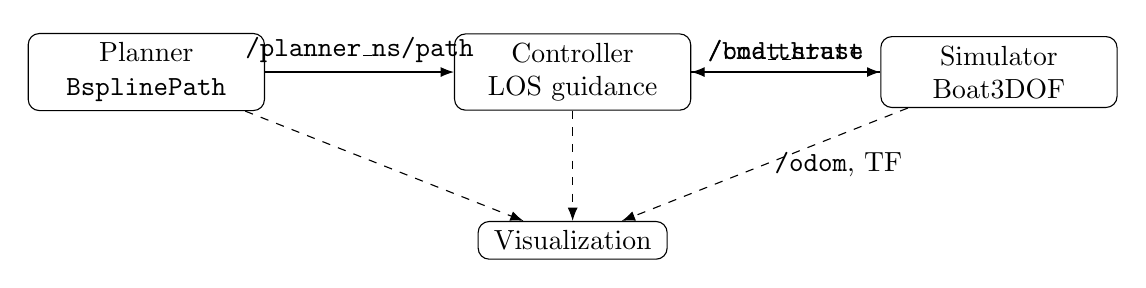
\begin{tikzpicture}[>=Latex,node distance=2.4cm]
    \node[draw,rounded corners,align=center,minimum width=3.0cm] (planner) {Planner\\\texttt{BsplinePath}};
    \node[draw,rounded corners,align=center,minimum width=3.0cm,right=of planner] (controller) {Controller\\LOS guidance};
    \node[draw,rounded corners,align=center,minimum width=3.0cm,right=of controller] (sim) {Simulator\\Boat3DOF};
    \node[draw,rounded corners,align=center,minimum width=2.4cm,below=1.4cm of controller] (viz) {Visualization};

    \draw[->] (planner) -- node[above] {\texttt{/planner\_ns/path}} (controller);
    \draw[->] (controller) -- node[above] {\texttt{/cmd\_thrust}} (sim);
    \draw[->] (sim) -- node[above] {\texttt{/boat\_state}} (controller);
    \draw[->,dashed] (sim) -- node[right] {\texttt{/odom}, TF} (viz);
    \draw[->,dashed] (planner) -- (viz);
    \draw[->,dashed] (controller) -- (viz);
  \end{tikzpicture}
  \caption{Data flow between the planner, controller, simulator, and visualization.}
  \label{fig:architecture}
\end{figure}

\section{Frames, signals, and conventions}
The simulator uses a planar world frame \emph{map} and a body frame \emph{base\_link}:
\begin{itemize}
  \item $x,y$ are inertial positions in the map frame (meters).
  \item $\psi$ is the heading/yaw angle (radians, CCW positive).
  \item $u,v$ are body-frame surge/sway velocities (m/s).
  \item $r$ is yaw rate (rad/s).
\end{itemize}

The actuator is a stern-mounted steerable rotor producing a thrust magnitude $T$
and an angle $\delta$ relative to body $+x$ (positive CCW). With a positive arm
$\ell > 0$ and the rotor located at $x=-\ell$, the yaw moment is
$N=-\ell\,T\sin\delta$, so positive $\delta$ produces a clockwise (negative) yaw
moment.

\subsection{Notation collisions}
The code uses $u$ for both surge velocity (a standard marine convention) and the
spline's internal unitless parameter. In the text we will write the spline
parameter as $u_{\mathrm{spline}}$ when needed; the arc-length parameter is
denoted $t$ (meters), consistent with \texttt{BSplinePath}.
\clearpage
\section{Planning (path generation)}
\subsection{Published message: \texttt{na\_msg/BsplinePath}}
The planner publishes a \texttt{BsplinePath} message consisting of parallel
arrays \texttt{ctrl\_x}, \texttt{ctrl\_y} (and \texttt{ctrl\_z}, currently always
zero). The controller requires:
\begin{itemize}
  \item at least 4 control points, and
  \item matching lengths for \texttt{ctrl\_x} and \texttt{ctrl\_y}.
\end{itemize}
The \texttt{closed} flag indicates whether indices wrap (closed loop) or clamp
at endpoints (open path). The message includes \texttt{degree} but the current
implementation always uses a uniform cubic spline, and therefore ignores
\texttt{degree}. The \texttt{start\_u} field provides an offset for the spline's
internal parameterization.

\subsection{Planner node (\texttt{planner\_node.py})}
The current ``planner'' is intentionally simple: it is a deterministic path
generator for closed-loop controller development. It publishes at a fixed timer
rate and selects a path using the parameter \texttt{path\_type}:
\begin{itemize}
  \item \texttt{CIRCLE}: a circle built from evenly spaced control points.
  \item \texttt{SQUARE\_SINUS}: a square-like loop with repeated corner points to
    adjust corner sharpness.
\end{itemize}

\subsection{Path alignment}
Before publishing, the planner aligns the path so runs start from a consistent
pose. The helper \texttt{\_align\_path\_to\_origin}:
\begin{enumerate}
  \item samples a closed spline preview,
  \item selects an ``anchor'' at approximately the lowest-$y$ sample,
  \item rotates the path so the local tangent points along $+x$, and
  \item translates the anchor to the origin.
\end{enumerate}
This keeps experiments repeatable across restarts.

\subsection{Uniform cubic B-spline representation}
The published control points are interpreted as a uniform cubic B-spline. The
code uses a unitless internal parameter $u_{\mathrm{spline}} = i + \tau$, where
$i=\lfloor u_{\mathrm{spline}} \rfloor$ and $\tau \in [0,1)$. The spline value is
\[
  \mathbf{C}(u_{\mathrm{spline}}) = b_0(\tau)\mathbf{P}_{i-1} + b_1(\tau)\mathbf{P}_{i}
  + b_2(\tau)\mathbf{P}_{i+1} + b_3(\tau)\mathbf{P}_{i+2},
\]
with basis functions:
\begin{align}
  b_0(\tau) &= \frac{-\tau^3 + 3\tau^2 - 3\tau + 1}{6}, &
  b_1(\tau) &= \frac{3\tau^3 - 6\tau^2 + 4}{6}, \\
  b_2(\tau) &= \frac{-3\tau^3 + 3\tau^2 + 3\tau + 1}{6}, &
  b_3(\tau) &= \frac{\tau^3}{6}.
\end{align}
For closed paths, indices wrap modulo $n$. For open paths, $u_{\mathrm{spline}}$
spans $[0,\,n-3]$ and clamps at the ends.

\subsection{Sampling and arc length}
\texttt{BSplinePath} samples the spline uniformly in $u_{\mathrm{spline}}$ and
accumulates Euclidean distances to approximate arc length $t$ (meters). The
sampled arrays provide fast conversions between $u_{\mathrm{spline}}$ and $t$.
The helper \texttt{samples\_from\_density} converts a \texttt{samples\_per\_meter}
tuning knob into a sample count by estimating the spline length from a coarse
preview.

\subsection{Planner parameters}
The planner currently exposes:
\begin{table}[h]
  \centering
  \begin{tabular}{@{}llll@{}}
    \toprule
    Parameter & Default & Units & Meaning \\
    \midrule
    \texttt{path\_type} & \texttt{SQUARE\_SINUS} & -- & Which demo path to publish \\
    \texttt{samples\_per\_meter} & 4.0 & \si{\per\meter} & Sampling density for preview + controller \\
    \bottomrule
  \end{tabular}
  \caption{Planner node parameters (see \texttt{planner\_node.py}).}
  \label{tab:planner_params}
\end{table}
\clearpage
\section{Control (LOS guidance)}
\subsection{Projection and Frenet frame}
The controller operates in the path's local Frenet frame, obtained by projecting
the boat position $(x,y)$ onto the spline. Projection is a two-stage process:
\begin{enumerate}
  \item Find the nearest sampled point (optionally within a window around a hint).
  \item Refine $u_{\mathrm{spline}}$ with a Gauss--Newton step along the spline tangent:
  \[
    \Delta u_{\mathrm{spline}} =
      \frac{(\mathbf{p}-\mathbf{C}(u_{\mathrm{spline}})) \cdot \mathbf{C}'(u_{\mathrm{spline}})}
      {\mathbf{C}'(u_{\mathrm{spline}})\cdot\mathbf{C}'(u_{\mathrm{spline}})}.
  \]
\end{enumerate}
The result provides a Frenet frame with unit tangent $\hat{\mathbf{t}}$,
unit normal $\hat{\mathbf{n}} = (-\hat{t}_y,\hat{t}_x)$ (left normal), and signed
cross-track error
\[
  cte = (\mathbf{p}-\mathbf{p}_{proj}) \cdot \hat{\mathbf{n}}.
\]
With this convention, $cte > 0$ means the boat is to the left of the path
tangent direction.

\subsection{\texttt{ProjectionTracker}}
\texttt{ProjectionTracker} adds state to stabilize sequential projections:
\begin{itemize}
  \item It keeps the last arc-length projection $t$.
  \item It predicts forward progress using body velocities and heading, by
    projecting the inertial velocity onto the path tangent.
  \item It limits jumps via \texttt{max\_jump} and can enforce minimum forward
    progress when the along-track speed is positive.
\end{itemize}
This reduces projection snapping on self-intersections but does not eliminate
all ambiguity.

\subsection{LOS guidance law}
The controller follows a line-of-sight (LOS) guidance pattern:
\begin{enumerate}
  \item If no valid spline is available, publish $[0,0]$ and exit.
  \item Project $(x,y)$ onto the path to get $t$, tangent, normal, and $cte$.
  \item Compute the path heading $\psi_{path}$ from the tangent; if the tangent
    norm is near zero, $\psi_{path}=0$.
  \item Choose a lookahead distance $L$ and advance to $t_{target}=t+L$.
  \item Compute desired heading
    \[
      \psi_d = \mathrm{wrap}\left(\psi_{path} - \arctan2(cte, L)\right).
    \]
  \item Apply a PD law on heading error with saturation:
    \[
      \delta = \mathrm{sat}\left(-k_p\,\mathrm{wrap}(\psi_d-\psi) - k_d\,r,\;\delta_{\max}\right).
    \]
  \item Thrust is constant: $T=\mathrm{sat}(T_0, T_{\max})$.
\end{enumerate}
The steering sign is consistent with the simulator's moment convention: positive
$\delta$ produces a negative yaw moment, so the controller uses a leading minus
sign in the PD law.

\subsection{Configuration parameters}
Default parameters live in \texttt{src/na\_launch/config/sim\_controller\_params.yaml}.
\texttt{config\_path} can override the YAML file for both simulator and controller.

\subsection{Controller parameters}
\begin{table}[h]
  \centering
  \begin{tabular}{@{}llll@{}}
    \toprule
    Parameter & Default & Units & Meaning \\
    \midrule
    \texttt{path\_topic} & \texttt{/planner\_ns/path} & -- & BsplinePath source \\
    \texttt{lookahead} & 4.0 & \si{\meter} & LOS lookahead distance \\
    \texttt{base\_thrust} & 15.0 & \si{\newton} & Constant thrust command \\
    \texttt{heading\_kp} & 2.0 & -- & Heading proportional gain \\
    \texttt{heading\_kd} & 0.5 & \si{\second} & Yaw-rate damping gain \\
    \texttt{max\_thrust} & 30.0 & \si{\newton} & Thrust saturation \\
    \texttt{max\_delta} & 1.570796 & \si{\radian} & Steering saturation \\
    \texttt{samples\_per\_meter} & 4.0 & \si{\per\meter} & B-spline sample density \\
    \texttt{max\_proj\_jump} & 0.2 & \si{\meter} & Projection jump limit \\
    \bottomrule
  \end{tabular}
  \caption{Controller tuning parameters and defaults.}
  \label{tab:controller_params}
\end{table}

\subsection{Examples and edge cases}
Figures in this section are generated from the same B-spline utilities used by
the controller. To refresh them, run
\texttt{latex/scripts/generate\_figures.py} and update the inline TikZ blocks in
this file.

\subsubsection{Example: closed-loop LOS tracking}
\Cref{fig:los_example} illustrates the projection, cross-track error, and
lookahead target on a closed spline generated from the same projection code.
\begin{figure}[h]
  \centering
% Auto-generated by latex/scripts/generate_figures.py
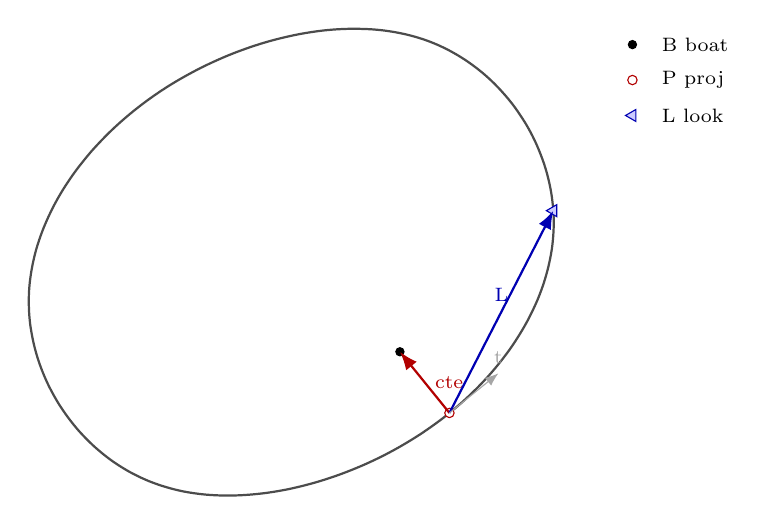
\begin{tikzpicture}[>=Latex,scale=1.0,every node/.style={font=\scriptsize}]
  \tikzset{
    path/.style={thick,black!70},
    cte/.style={red!70!black,thick,->},
    look/.style={blue!70!black,thick,->},
    tan/.style={gray!70,->},
    boat/.style={circle,fill=black,inner sep=1.2pt},
    proj/.style={circle,draw=red!70!black,fill=white,inner sep=1.2pt},
    lookahead/.style={regular polygon,regular polygon sides=3,draw=blue!70!black,fill=blue!20,minimum size=5pt,inner sep=0pt,rotate=90}
  }
  \draw[path] plot [smooth cycle] coordinates { (0.333,0.667) (0.471,0.626) (0.612,0.592) (0.756,0.567) (0.903,0.549) (1.053,0.539) (1.205,0.536) (1.359,0.540) (1.515,0.551) (1.672,0.568) (1.829,0.592) (1.987,0.622) (2.145,0.659) (2.302,0.701) (2.459,0.749) (2.615,0.803) (2.769,0.862) (2.922,0.926) (3.072,0.995) (3.220,1.069) (3.365,1.148) (3.506,1.231) (3.644,1.318) (3.778,1.410) (3.908,1.505) (4.033,1.605) (4.154,1.707) (4.270,1.814) (4.381,1.923) (4.487,2.035) (4.587,2.150) (4.682,2.268) (4.772,2.388) (4.855,2.511) (4.932,2.635) (5.004,2.762) (5.068,2.890) (5.127,3.020) (5.178,3.151) (5.222,3.283) (5.259,3.416) (5.289,3.550) (5.312,3.685) (5.326,3.820) (5.333,3.955) (5.332,4.090) (5.322,4.225) (5.305,4.360) (5.280,4.493) (5.248,4.625) (5.208,4.756) (5.161,4.884) (5.108,5.010) (5.048,5.133) (4.981,5.253) (4.907,5.369) (4.828,5.482) (4.742,5.590) (4.651,5.693) (4.554,5.792) (4.452,5.885) (4.344,5.972) (4.232,6.053) (4.114,6.128) (3.992,6.196) (3.865,6.257) (3.734,6.310) (3.598,6.355) (3.459,6.392) (3.317,6.421) (3.171,6.443) (3.022,6.457) (2.871,6.463) (2.718,6.463) (2.563,6.456) (2.407,6.442) (2.250,6.421) (2.092,6.394) (1.934,6.360) (1.776,6.321) (1.619,6.276) (1.463,6.225) (1.308,6.169) (1.154,6.107) (1.003,6.040) (0.854,5.969) (0.708,5.892) (0.564,5.811) (0.424,5.726) (0.288,5.636) (0.157,5.543) (0.029,5.445) (-0.094,5.344) (-0.212,5.240) (-0.326,5.132) (-0.434,5.021) (-0.538,4.908) (-0.635,4.791) (-0.728,4.672) (-0.814,4.551) (-0.895,4.427) (-0.969,4.302) (-1.037,4.174) (-1.098,4.045) (-1.153,3.915) (-1.201,3.783) (-1.242,3.651) (-1.275,3.517) (-1.301,3.383) (-1.320,3.248) (-1.331,3.113) (-1.333,2.977) (-1.328,2.842) (-1.315,2.707) (-1.293,2.573) (-1.265,2.441) (-1.229,2.309) (-1.186,2.180) (-1.136,2.053) (-1.079,1.928) (-1.015,1.807) (-0.945,1.688) (-0.868,1.574) (-0.786,1.464) (-0.698,1.358) (-0.603,1.257) (-0.504,1.161) (-0.399,1.071) (-0.289,0.986) (-0.173,0.908) (-0.054,0.837) (0.071,0.773) (0.200,0.716) (0.333,0.667) };
  \coordinate (boat) at (3.380,2.362);
  \coordinate (proj) at (4.009,1.585);
  \coordinate (target) at (5.328,4.154);
  \coordinate (tan) at (4.631,2.088);
  \node[boat] at (boat) {};
  \node[proj] at (proj) {};
  \node[lookahead] at (target) {};
  \draw[cte] (proj) -- (boat) node[midway,right] {cte};
  \draw[look] (proj) -- (target) node[midway,above] {L};
  \draw[tan] (proj) -- (tan) node[above] {t};
  \node[boat] at (6.333,6.263) {};
  \node[anchor=west] at (6.583,6.263) {B boat};
  \node[proj] at (6.333,5.813) {};
  \node[anchor=west] at (6.583,5.813) {P proj};
  \node[lookahead] at (6.333,5.363) {};
  \node[anchor=west] at (6.583,5.363) {L look};
\end{tikzpicture}
  \caption{LOS tracking geometry on a closed spline generated from the path utilities (B: boat, P: projection, L: lookahead).}
  \label{fig:los_example}
\end{figure}

\subsubsection{Example: open path end behavior}
\Cref{fig:open_end} shows an open path with the vessel near the end. The
lookahead point clamps at the end of the spline; there is no wrap-around.
\begin{figure}[h]
  \centering
% Auto-generated by latex/scripts/generate_figures.py
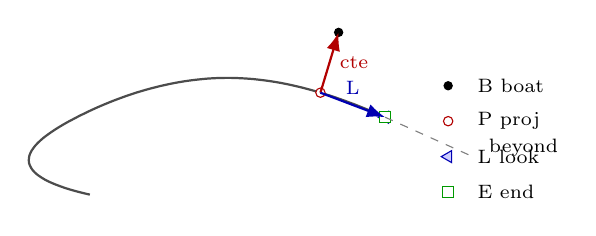
\begin{tikzpicture}[>=Latex,scale=1.0,every node/.style={font=\scriptsize}]
  \tikzset{
    path/.style={thick,black!70},
    cte/.style={red!70!black,thick,->},
    look/.style={blue!70!black,thick,->},
    boat/.style={circle,fill=black,inner sep=1.2pt},
    proj/.style={circle,draw=red!70!black,fill=white,inner sep=1.2pt},
    lookahead/.style={regular polygon,regular polygon sides=3,draw=blue!70!black,fill=blue!20,minimum size=5pt,inner sep=0pt,rotate=90},
    endpt/.style={rectangle,draw=green!60!black,fill=white,minimum size=4pt,inner sep=0pt}
  }
  \draw[path] plot [smooth] coordinates { (-2.250,0.117) (-2.358,0.143) (-2.457,0.169) (-2.547,0.196) (-2.628,0.224) (-2.701,0.252) (-2.766,0.280) (-2.823,0.309) (-2.872,0.339) (-2.914,0.368) (-2.949,0.398) (-2.977,0.429) (-2.998,0.459) (-3.013,0.490) (-3.023,0.521) (-3.026,0.552) (-3.024,0.583) (-3.018,0.614) (-3.006,0.645) (-2.989,0.677) (-2.968,0.708) (-2.944,0.739) (-2.915,0.770) (-2.883,0.801) (-2.848,0.832) (-2.809,0.862) (-2.768,0.892) (-2.725,0.922) (-2.679,0.952) (-2.632,0.981) (-2.583,1.010) (-2.532,1.039) (-2.481,1.066) (-2.428,1.094) (-2.376,1.121) (-2.322,1.147) (-2.269,1.173) (-2.215,1.198) (-2.160,1.223) (-2.105,1.247) (-2.050,1.270) (-1.994,1.293) (-1.938,1.315) (-1.882,1.336) (-1.825,1.357) (-1.769,1.377) (-1.711,1.396) (-1.654,1.415) (-1.596,1.432) (-1.538,1.449) (-1.480,1.465) (-1.421,1.480) (-1.363,1.495) (-1.304,1.508) (-1.245,1.521) (-1.186,1.533) (-1.126,1.544) (-1.067,1.554) (-1.007,1.563) (-0.947,1.571) (-0.887,1.578) (-0.827,1.584) (-0.767,1.590) (-0.707,1.594) (-0.647,1.597) (-0.587,1.599) (-0.527,1.600) (-0.467,1.600) (-0.406,1.599) (-0.346,1.596) (-0.286,1.593) (-0.226,1.589) (-0.166,1.584) (-0.105,1.577) (-0.045,1.570) (0.015,1.562) (0.075,1.553) (0.135,1.543) (0.196,1.532) (0.256,1.520) (0.316,1.507) (0.376,1.493) (0.436,1.479) (0.497,1.463) (0.557,1.447) (0.617,1.430) (0.677,1.413) (0.737,1.394) (0.798,1.375) (0.858,1.355) (0.918,1.334) (0.978,1.313) (1.038,1.290) (1.099,1.268) (1.159,1.244) (1.219,1.220) (1.279,1.196) (1.339,1.170) (1.400,1.144) (1.460,1.118) (1.500,1.100) };
  \coordinate (boat) at (0.909,2.178);
  \coordinate (proj) at (0.678,1.412);
  \coordinate (target) at (1.500,1.100);
  \coordinate (endpt) at (1.500,1.100);
  \coordinate (beyond) at (2.594,0.608);
  \node[boat] at (boat) {};
  \node[proj] at (proj) {};
  \node[lookahead] at (target) {};
  \node[endpt] at (endpt) {};
  \draw[cte] (proj) -- (boat) node[midway,right] {cte};
  \draw[look] (proj) -- (target) node[midway,above] {L};
  \draw[dashed,gray] (endpt) -- (beyond);
  \node[anchor=west] at (2.694,0.708) {beyond};
  \node[boat] at (2.300,1.500) {};
  \node[anchor=west] at (2.550,1.500) {B boat};
  \node[proj] at (2.300,1.050) {};
  \node[anchor=west] at (2.550,1.050) {P proj};
  \node[lookahead] at (2.300,0.600) {};
  \node[anchor=west] at (2.550,0.600) {L look};
  \node[endpt] at (2.300,0.150) {};
  \node[anchor=west] at (2.550,0.150) {E end};
\end{tikzpicture}
  \caption{Open-path end behavior: \texttt{advance\_t} clamps instead of wrapping (B: boat, P: projection, L: lookahead, E: end).}
  \label{fig:open_end}
\end{figure}

\subsubsection{Edge case: sparse sampling}
\Cref{fig:sampling_density} compares a dense spline sample to a coarse sample
count. Sparse samples reduce projection accuracy and can create large $cte$
discontinuities.
\begin{figure}[h]
  \centering
% Auto-generated by latex/scripts/generate_figures.py
\begin{tikzpicture}[>=Latex,scale=0.95,every node/.style={font=\scriptsize}]
  \tikzset{
    finepath/.style={thick,black!70},
    coarsepath/.style={orange!80!black,dashed},
    coarsept/.style={circle,draw=orange!80!black,fill=orange!40,inner sep=0.6pt}
  }
  \draw[finepath] plot [smooth cycle] coordinates { (-3.667,0.000) (-3.664,0.100) (-3.657,0.200) (-3.645,0.300) (-3.628,0.400) (-3.606,0.499) (-3.581,0.597) (-3.551,0.695) (-3.517,0.791) (-3.478,0.887) (-3.436,0.982) (-3.391,1.075) (-3.341,1.167) (-3.288,1.257) (-3.232,1.346) (-3.172,1.433) (-3.109,1.518) (-3.044,1.601) (-2.975,1.682) (-2.904,1.761) (-2.830,1.837) (-2.753,1.911) (-2.674,1.982) (-2.593,2.051) (-2.510,2.117) (-2.424,2.181) (-2.337,2.242) (-2.248,2.301) (-2.158,2.357) (-2.066,2.411) (-1.972,2.462) (-1.877,2.511) (-1.782,2.557) (-1.685,2.601) (-1.587,2.642) (-1.489,2.680) (-1.390,2.716) (-1.290,2.750) (-1.190,2.781) (-1.090,2.810) (-0.990,2.836) (-0.890,2.859) (-0.789,2.880) (-0.689,2.899) (-0.589,2.915) (-0.489,2.928) (-0.388,2.939) (-0.288,2.948) (-0.188,2.954) (-0.088,2.957) (0.013,2.958) (0.113,2.957) (0.213,2.953) (0.313,2.946) (0.414,2.937) (0.514,2.925) (0.614,2.911) (0.714,2.895) (0.815,2.875) (0.915,2.854) (1.015,2.830) (1.115,2.803) (1.215,2.774) (1.315,2.742) (1.415,2.708) (1.513,2.671) (1.612,2.632) (1.709,2.590) (1.806,2.546) (1.901,2.499) (1.996,2.450) (2.089,2.398) (2.180,2.343) (2.271,2.287) (2.359,2.227) (2.446,2.165) (2.531,2.101) (2.613,2.034) (2.694,1.965) (2.772,1.893) (2.848,1.818) (2.922,1.741) (2.992,1.662) (3.060,1.581) (3.125,1.497) (3.187,1.411) (3.246,1.324) (3.302,1.235) (3.354,1.144) (3.402,1.052) (3.447,0.958) (3.488,0.863) (3.526,0.767) (3.559,0.670) (3.588,0.572) (3.612,0.474) (3.632,0.375) (3.648,0.275) (3.659,0.175) (3.665,0.075) (3.667,-0.025) (3.663,-0.125) (3.654,-0.225) (3.641,-0.325) (3.623,-0.424) (3.600,-0.523) (3.574,-0.621) (3.543,-0.719) (3.507,-0.815) (3.468,-0.911) (3.425,-1.005) (3.379,-1.098) (3.328,-1.189) (3.274,-1.279) (3.217,-1.368) (3.157,-1.454) (3.093,-1.539) (3.027,-1.622) (2.957,-1.702) (2.885,-1.780) (2.811,-1.856) (2.734,-1.929) (2.654,-2.000) (2.572,-2.068) (2.488,-2.133) (2.403,-2.197) (2.315,-2.257) (2.226,-2.315) (2.135,-2.371) (2.042,-2.424) (1.949,-2.474) (1.854,-2.523) (1.758,-2.568) (1.660,-2.611) (1.563,-2.652) (1.464,-2.690) (1.365,-2.725) (1.265,-2.758) (1.165,-2.789) (1.065,-2.817) (0.965,-2.842) (0.865,-2.865) (0.764,-2.885) (0.664,-2.903) (0.564,-2.919) (0.464,-2.931) (0.363,-2.942) (0.263,-2.950) (0.163,-2.955) (0.063,-2.958) (-0.038,-2.958) (-0.138,-2.956) (-0.238,-2.951) (-0.338,-2.944) (-0.439,-2.934) (-0.539,-2.922) (-0.639,-2.907) (-0.739,-2.890) (-0.840,-2.870) (-0.940,-2.848) (-1.040,-2.823) (-1.140,-2.796) (-1.240,-2.766) (-1.340,-2.734) (-1.439,-2.699) (-1.538,-2.661) (-1.636,-2.621) (-1.733,-2.579) (-1.830,-2.534) (-1.925,-2.487) (-2.019,-2.437) (-2.112,-2.384) (-2.203,-2.329) (-2.293,-2.272) (-2.381,-2.212) (-2.467,-2.149) (-2.552,-2.084) (-2.634,-2.017) (-2.714,-1.947) (-2.792,-1.874) (-2.867,-1.799) (-2.940,-1.722) (-3.010,-1.642) (-3.077,-1.560) (-3.141,-1.476) (-3.202,-1.390) (-3.260,-1.302) (-3.315,-1.212) (-3.366,-1.121) (-3.414,-1.028) (-3.458,-0.934) (-3.498,-0.839) (-3.534,-0.743) (-3.566,-0.646) (-3.594,-0.548) (-3.618,-0.449) (-3.637,-0.350) (-3.651,-0.250) (-3.661,-0.150) (-3.666,-0.050) (-3.667,0.000) };
  \draw[coarsepath] plot [smooth cycle] coordinates { (-3.667,0.000) (-3.555,0.683) (-3.246,1.325) (-2.781,1.884) (-2.202,2.330) (-1.548,2.657) (-0.862,2.865) (-0.172,2.955) (0.517,2.925) (1.207,2.776) (1.882,2.509) (2.503,2.122) (3.030,1.617) (3.422,1.011) (3.638,0.344) (3.638,-0.344) (3.422,-1.011) (3.030,-1.617) (2.503,-2.122) (1.882,-2.509) (1.207,-2.776) (0.517,-2.925) (-0.172,-2.955) (-0.862,-2.865) (-1.548,-2.657) (-2.202,-2.330) (-2.781,-1.884) (-3.246,-1.325) (-3.555,-0.683) (-3.667,0.000) };
  \foreach \p in {(-3.667,0.000), (-3.555,0.683), (-3.246,1.325), (-2.781,1.884), (-2.202,2.330), (-1.548,2.657), (-0.862,2.865), (-0.172,2.955), (0.517,2.925), (1.207,2.776), (1.882,2.509), (2.503,2.122), (3.030,1.617), (3.422,1.011), (3.638,0.344), (3.638,-0.344), (3.422,-1.011), (3.030,-1.617), (2.503,-2.122), (1.882,-2.509), (1.207,-2.776), (0.517,-2.925), (-0.172,-2.955), (-0.862,-2.865), (-1.548,-2.657), (-2.202,-2.330), (-2.781,-1.884), (-3.246,-1.325), (-3.555,-0.683), (-3.667,0.000)} { \node[coarsept] at \p {}; }
  \draw[finepath] (3.367,2.758) -- (3.967,2.758);
  \node[anchor=west] at (4.317,2.758) {fine path};
  \draw[coarsepath] (3.367,2.308) -- (3.967,2.308);
  \node[anchor=west] at (4.317,2.308) {coarse path};
  \node[coarsept] at (3.667,1.858) {};
  \node[anchor=west] at (4.317,1.858) {samples};
\end{tikzpicture}
  \caption{Effect of low sampling density on the spline representation (coarse samples shown as points).}
  \label{fig:sampling_density}
\end{figure}

\subsubsection{Expected behavior}
\begin{itemize}
  \item Fewer than 4 control points or mismatched \texttt{ctrl\_x}/\texttt{ctrl\_y} arrays:
    controller rejects the path, outputs $[0,0]$, and resets projection history.
  \item Very low \texttt{samples\_per\_meter} (or non-positive values): the spline is
    still built but with coarse sampling, which degrades projection accuracy (see
    \Cref{fig:sampling_density}).
  \item Self-intersections or tight loops: multiple projections can be locally optimal.
    \texttt{max\_proj\_jump} helps, but jumps are still possible with sharp geometry.
  \item Tangent norm near zero (repeated control points): heading defaults to 0,
    so steering may be arbitrary until geometry improves.
  \item Extremely small lookahead: high steering activity and oscillation.
    Extremely large lookahead: slow convergence and large steady-state $cte$.
\end{itemize}
\clearpage
\section{Simulator}
\subsection{Three Degree of Freedom Vessel Model}

\subsubsection{Motivation and Scope}
This simulator models the motion of a small surface vessel in two dimensions, focusing on its behavior in the horizontal plane. For tasks such as path following, obstacle avoidance, and low-speed maneuvering, the dominant dynamics are those governing planar motion—namely translation in the forward and lateral directions, and rotation about the vertical axis. Vertical motion and angular attitude dynamics (heave, roll, and pitch) are typically negligible in this regime and are therefore excluded for simplicity.

We adopt a classical three degree of freedom (3 DOF) rigid body model capturing surge (forward motion), sway (sideways motion), and yaw (heading rate). This model serves as a physically meaningful baseline that is easy to implement, fast to simulate, and compatible with later extensions to full six degree of freedom models.

\subsubsection{Coordinate Frames}
We define two coordinate frames:
\begin{itemize}
  \item The \textbf{world frame} $\{W\}$ is a fixed inertial frame with horizontal axes $x$ and $y$, and vertical axis $z$ pointing upward.
  \item The \textbf{body frame} $\{B\}$ is attached to the vessel at its center of gravity. The body $x$ axis points forward along the vessel's longitudinal axis, the $y$ axis points to starboard, and the $z$ axis points downward, following the marine convention.
\end{itemize}

The vessel's heading angle $\psi$ defines the rotation of the body frame relative to the world frame, measured from the world $x$ axis to the body $x$ axis in the horizontal plane.

\subsubsection{Degrees of Freedom: Surge, Sway, and Yaw}
The motion of the vessel is described using three degrees of freedom:
\begin{itemize}
  \item \textbf{Surge} (\( u \)) is the translational velocity in the forward direction (along the body $x$ axis).
  \item \textbf{Sway} (\( v \)) is the lateral velocity toward starboard (along the body $y$ axis).
  \item \textbf{Yaw} (\( r \)) is the angular velocity about the vertical axis (body $z$ axis), corresponding to changes in heading.
\end{itemize}

These three motions define the 3 DOF configuration of the vessel in the horizontal plane.

\subsubsection{State Variables}
The vessel state is split into pose and velocity:
\begin{align*}
\boldsymbol{\eta} &=
\begin{bmatrix}
x \\ y \\ \psi
\end{bmatrix}, \quad \text{position and heading in world frame}, \\
\boldsymbol{\nu} &=
\begin{bmatrix}
u \\ v \\ r
\end{bmatrix}, \quad \text{velocities in body frame}.
\end{align*}
The complete simulator state vector is:
\[
\mathbf{x} =
\begin{bmatrix}
\boldsymbol{\eta} \\
\boldsymbol{\nu}
\end{bmatrix}
=
\begin{bmatrix}
x \\ y \\ \psi \\ u \\ v \\ r
\end{bmatrix}.
\]

\subsubsection{Kinematics}
To relate body-frame velocities to changes in world-frame position, we use a rotation matrix:
\[
\mathbf{R}(\psi) =
\begin{bmatrix}
\cos\psi & -\sin\psi & 0 \\
\sin\psi &  \cos\psi & 0 \\
0        &  0        & 1
\end{bmatrix}.
\]
The kinematic equations are:
\[
\dot{\boldsymbol{\eta}} = \mathbf{R}(\psi)\boldsymbol{\nu},
\]
which yields:
\begin{align}
\dot{x} &= u\cos\psi - v\sin\psi, \\
\dot{y} &= u\sin\psi + v\cos\psi, \\
\dot{\psi} &= r.
\end{align}

\subsubsection{Actuation and Force Mapping}
The vessel is actuated by a single steerable rotor located at a distance \( \ell \) behind the center of gravity, along the body $x$ axis. The control inputs are:
\begin{itemize}
  \item \( T \in \mathbb{R} \): thrust magnitude,
  \item \( \delta \in \mathbb{R} \): steering angle relative to the body $x$ axis.
\end{itemize}

The thrust vector in the body frame is:
\[
\mathbf{f}_T =
\begin{bmatrix}
T\cos\delta \\
T\sin\delta \\
0
\end{bmatrix}.
\]

The generalized force components become:
\begin{align}
X &= T\cos\delta, \quad \text{(surge)} \\
Y &= T\sin\delta, \quad \text{(sway)} \\
N &= -\ell \cdot Y = -\ell T \sin\delta, \quad \text{(yaw moment)}.
\end{align}

\subsubsection{Rigid Body Dynamics}
We apply Newton–Euler equations in the body frame.

\paragraph{Linear Momentum}
The vessel has linear momentum
\[
\mathbf{p} = m
\begin{bmatrix}
u \\ v \\ 0
\end{bmatrix},
\]
and angular velocity
\[
\boldsymbol{\omega} =
\begin{bmatrix}
0 \\ 0 \\ r
\end{bmatrix}.
\]

The body-frame form of Newton's second law is:
\[
\dot{\mathbf{p}} + \boldsymbol{\omega} \times \mathbf{p} = \mathbf{f}.
\]
The cross product yields:
\[
\boldsymbol{\omega} \times \mathbf{p} =
\begin{bmatrix}
-mvr \\
mur \\
0
\end{bmatrix}.
\]

Substituting gives:
\begin{align}
m\dot{u} - mvr &= X, \\
m\dot{v} + mur &= Y.
\end{align}

\paragraph{Angular Momentum}
For yaw, we have:
\[
I_z \dot{r} = N.
\]

\subsubsection{Hydrodynamic Damping and Linearization}
The surrounding water exerts resistive forces that oppose motion. These forces depend on the vessel velocity and are modeled using linear and quadratic damping terms.

\paragraph{Surge damping} is modeled as:
\[
X_D = -X_u u - X_{uu} |u|u,
\]
where:
\begin{itemize}
  \item \( X_u \) is the linear surge damping coefficient,
  \item \( X_{uu} \) is the quadratic surge damping coefficient.
\end{itemize}
The total surge force is then:
\[
X = T\cos\delta + X_D = T\cos\delta - X_u u - X_{uu}|u|u.
\]

\paragraph{Substitution into equations of motion}
The full surge equation becomes:
\[
m\dot{u} - mvr = T\cos\delta - X_u u - X_{uu}|u|u,
\]
so that:
\[
\dot{u} = \frac{1}{m} \left( T\cos\delta - X_u u - X_{uu} |u|u + mvr \right).
\]

\paragraph{Sway and yaw damping} are similarly modeled as:
\begin{align*}
Y_D &= -Y_v v - Y_r r, \\
N_D &= -N_v v - N_r r,
\end{align*}
and included in the equations:
\begin{align}
\dot{v} &= \frac{1}{m} \left( T\sin\delta - Y_v v - Y_r r - mur \right), \\
\dot{r} &= \frac{1}{I_z} \left( -\ell T \sin\delta - N_v v - N_r r \right).
\end{align}

\paragraph{Linearization}
For small velocities, we can approximate:
\[
X_D \approx -X_u u,
\]
since \( |u|u \approx 0 \) near \( u = 0 \). This gives a linear damping model:
\[
m\dot{u} - mvr \approx T\cos\delta - X_u u.
\]

This is useful in linear control design (e.g. LQR). For higher speeds, the full nonlinear damping model must be retained.

\paragraph{Example}
Let:
\[
X_u = 5.0, \quad X_{uu} = 1.0, \quad u = 2.0 \, \si{m/s}.
\]
Then:
\[
X_D = -5\cdot 2 - 1\cdot |2|\cdot 2 = -10 - 4 = -14 \, \si{N}.
\]

\subsubsection{Final Model Summary}
The complete 3 DOF model consists of:
\begin{itemize}
  \item Kinematic equations:
  \[
  \begin{aligned}
  \dot{x} &= u\cos\psi - v\sin\psi, \\
  \dot{y} &= u\sin\psi + v\cos\psi, \\
  \dot{\psi} &= r,
  \end{aligned}
  \]
  \item Dynamic equations with damping:
  \[
  \begin{aligned}
  \dot{u} &= \frac{1}{m} \left( T\cos\delta - X_u u - X_{uu}|u|u + mvr \right), \\
  \dot{v} &= \frac{1}{m} \left( T\sin\delta - Y_v v - Y_r r - mur \right), \\
  \dot{r} &= \frac{1}{I_z} \left( -\ell T \sin\delta - N_v v - N_r r \right).
  \end{aligned}
  \]
\end{itemize}

\subsubsection{Relation to 6 DOF Models}
This 3 DOF model is a direct restriction of the full 6 DOF marine craft dynamics, obtained by setting:
\[
z = \phi = \theta = 0, \qquad w = p = q = 0,
\]
and neglecting the associated forces and moments. The same coordinate frames and notational structure are retained, which allows the model to be upgraded to higher fidelity without rederiving the formulation.

\subsection{Simulation node (\texttt{sim\_node.py})}
The simulator node integrates the continuous-time ODE using RK4 with timestep
\texttt{dt}. Inputs are saturated to
$(T,\delta)\in[-T_{\max},T_{\max}]\times[-\delta_{\max},\delta_{\max}]$ and can
be rate-limited in $\delta$ via \texttt{max\_delta\_rate}. Commands are held at
the last received value.

\subsubsection{Outputs}
The simulator publishes:
\begin{itemize}
  \item \texttt{/boat\_state} with $[x,y,\psi,u,v,r]$.
  \item \texttt{/odom} with position, yaw-only quaternion, and twist.
  \item TF transform \texttt{map} $\rightarrow$ \texttt{base\_link}.
\end{itemize}

\subsection{Simulator parameters}
\begin{table}[h]
  \centering
  \begin{tabular}{@{}llll@{}}
    \toprule
    Parameter & Default & Units & Meaning \\
    \midrule
    \texttt{m} & 70.0 & \si{\kilogram} & Mass \\
    \texttt{Iz} & 10.0 & \si{\kilogram\meter\squared} & Yaw inertia \\
    \texttt{Xu} & 5.0 & -- & Linear surge damping \\
    \texttt{Xuu} & 1.0 & -- & Quadratic surge damping \\
    \texttt{Yv} & 40.0 & -- & Linear sway damping \\
    \texttt{Yr} & 5.0 & -- & Yaw-rate to sway coupling \\
    \texttt{Nv} & 5.0 & -- & Yaw moment from sway velocity \\
    \texttt{Nr} & 40.0 & -- & Yaw rotational damping \\
    \texttt{l} & 0.5 & \si{\meter} & Rotor arm (positive scalar) \\
    \texttt{dt} & 0.02 & \si{\second} & Integration step \\
    \texttt{max\_thrust} & 40.0 & \si{\newton} & Thrust saturation \\
    \texttt{max\_delta} & 1.570796 & \si{\radian} & Steering saturation \\
    \texttt{max\_delta\_rate} & 0.0 & \si{\radian\per\second} & Steering rate limit \\
    \bottomrule
  \end{tabular}
  \caption{Simulator parameters and defaults.}
  \label{tab:sim_params}
\end{table}
\clearpage
\section{Design intent, expectations, and limitations}
\subsection{Purpose}
The current setup is intentionally simple: a deterministic closed loop for
testing planning (path generation), LOS guidance, and simulation without heavy
dependencies.

\subsection{What we expect}
\begin{itemize}
  \item With smooth paths and reasonable lookahead, the vessel should converge
    to the path and maintain bounded $cte$.
  \item Heading error should be damped by the $k_d r$ term without large overshoot.
  \item Projection should remain stable on benign paths when \texttt{max\_proj\_jump}
    is smaller than the local path curvature radius.
\end{itemize}

\subsection{Limitations and risks}
\begin{itemize}
  \item The controller uses constant thrust and no speed regulation; path tracking
    quality depends strongly on the chosen thrust and vessel damping.
  \item The projection is sample-based and approximate; performance degrades on
    sparse samples or sharp corners.
  \item Open paths are not decelerated near the end; without external logic, the
    vessel will keep pushing past the terminal point.
  \item \texttt{max\_proj\_jump} trades stability for reacquisition; values that are
    too small can prevent convergence after large jumps or path switches.
  \item The \texttt{BsplinePath} message includes \texttt{degree} and \texttt{ctrl\_z}
    fields, but the current implementation ignores them.
  \item \texttt{Float32MultiArray} topics lack explicit timestamps or frames, which
    limits synchronization in real systems.
  \item \texttt{/boat\_state} and \texttt{/cmd\_thrust} are absolute topic names, so
    namespacing requires explicit remapping for multi-vehicle setups.
  \item The simulator is planar with simplified damping and no environmental effects;
    it is not a high-fidelity hydrodynamic model.
  \item Automated tests exist for the B-spline utilities, but the controller and
    simulator currently lack direct unit tests.
\end{itemize}

\section{How this stays in sync with code}
The most detailed source of truth is the implementation itself. To keep this
document aligned with the code:
\begin{itemize}
  \item Update equations here when you change \texttt{Boat3DOF.dynamics()}.
  \item Update the controller logic when you change \texttt{ControllerNode.control\_loop()}.
  \item Update the planner section when you change \texttt{PlannerPublisher}.
  \item Update the spline section when you change \texttt{BSplinePath} or
    \texttt{ProjectionTracker}.
  \item Keep parameter tables aligned with \texttt{sim\_controller\_params.yaml}.
  \item When projection or sampling changes, regenerate figures with
    \texttt{latex/scripts/generate\_figures.py} and update the inline TikZ blocks
    in this file.
  \item Refresh example figures if coordinate conventions or sign choices change.
\end{itemize}

\end{document}
